\section{Shape Class Reference}
\label{classShape}\index{Shape@{Shape}}
Inheritance diagram for Shape::\begin{figure}[H]
\begin{center}
\leavevmode
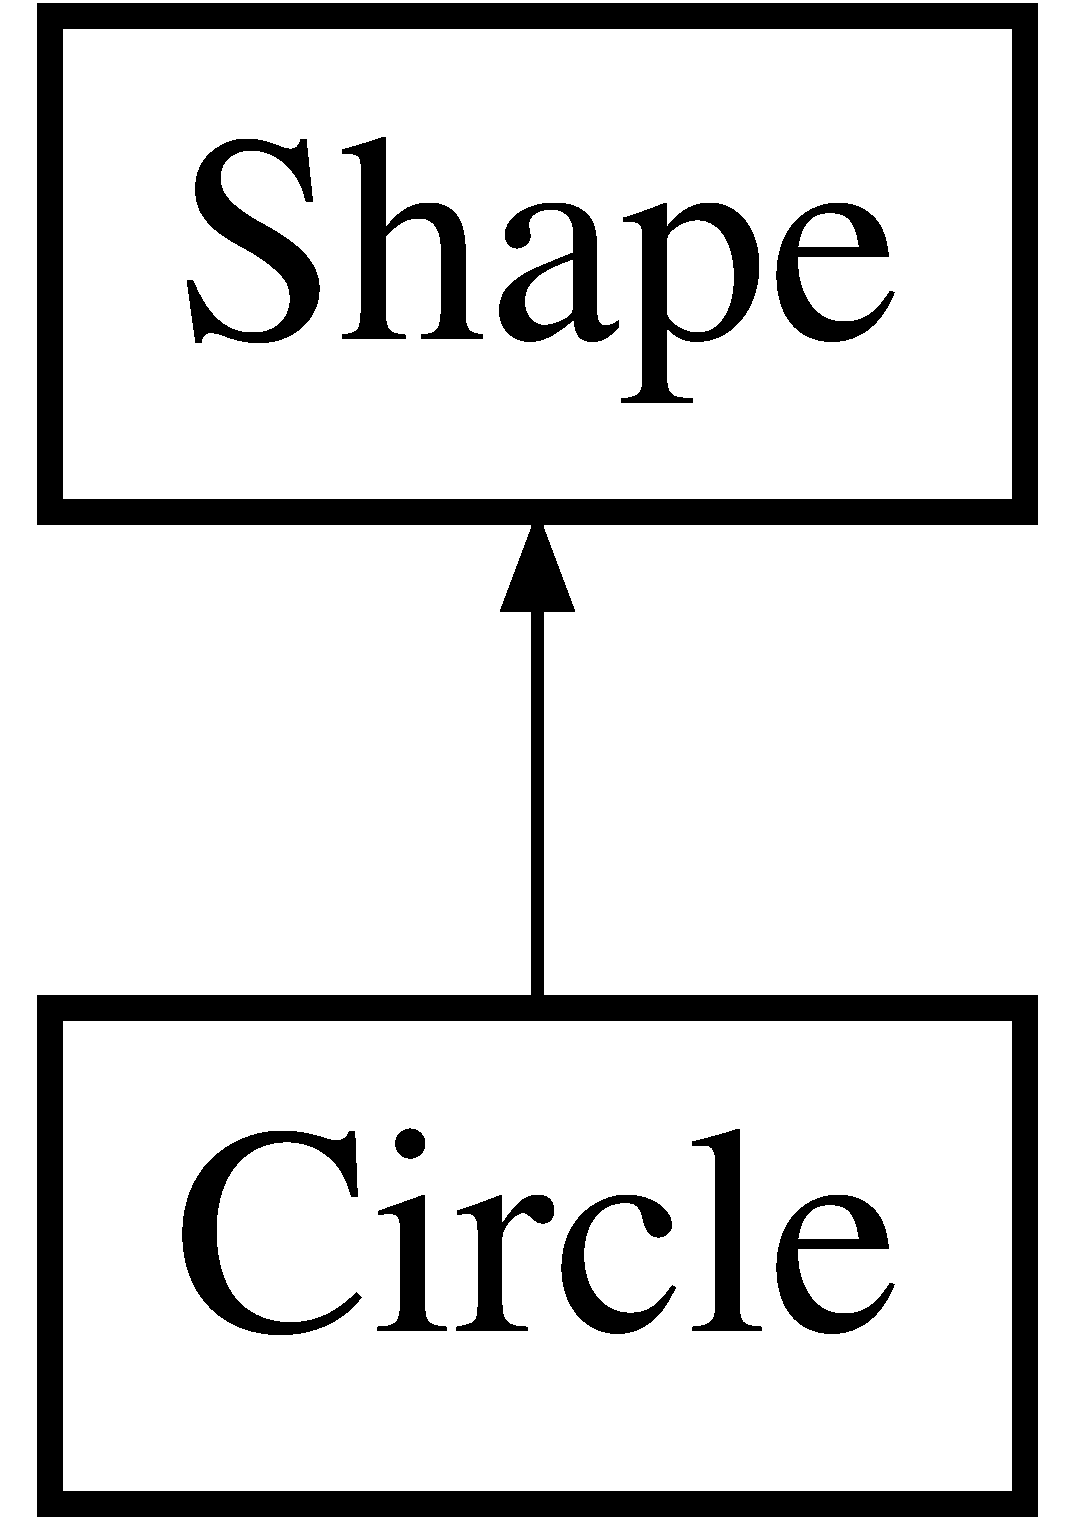
\includegraphics[height=2cm]{classShape}
\end{center}
\end{figure}
\subsection*{Public Member Functions}
\begin{CompactItemize}
\item 
abstract Number {\bf get\-Area} ()\label{classShape_8ae6f32689d68a8b9d93ebf22cc03f26}

\end{CompactItemize}


\subsection{Detailed Description}




Definition at line 17 of file Test\-Return\-Inheritance.java.

The documentation for this class was generated from the following file:\begin{CompactItemize}
\item 
Test\-Return\-Inheritance.java\end{CompactItemize}
